\documentclass[11pt,letterpaper]{article}
\usepackage{fontspec}
\setmainfont{texgyrepagella}[Extension=.otf,UprightFont=*-regular,BoldFont=*-bold,ItalicFont=*-italic,BoldItalicFont=*-bolditalic]
\usepackage[bidi=default]{babel}
\babelprovide[import,main]{spanish}
\babelprovide[import]{hebrew}
\babelprovide[import]{ancientgreek}
\babelfont[hebrew]{rm}[Path=fonts/,BoldFont=NotoHebrewSerif-700.ttf,Scale=0.95]{NotoHebrewSerif-400.ttf}
\babelfont[ancientgreek]{rm}[Path=fonts/]{GFSPorson.otf}
\newcommand{\heb}[1]{\mbox{\foreignlanguage{hebrew}{#1}}}
\newcommand{\grc}[1]{\foreignlanguage{ancientgreek}{#1}}
\newcommand{\hebverso}[1]{\par\smallskip{\centering\begin{otherlanguage}{hebrew}\large #1\end{otherlanguage}\par}\smallskip}
\newcommand{\SENOR}{\textsc{Señor}}
\usepackage[margin=2.5cm,headheight=14pt]{geometry}
\usepackage{microtype,ragged2e,booktabs,graphicx,xcolor,csquotes,array}
\usepackage[hidelinks]{hyperref}\usepackage{xurl}\urlstyle{same}
\usepackage[most]{tcolorbox}
\usepackage{tikz}\usetikzlibrary{arrows.meta,positioning,calc,decorations.pathreplacing}
\usepackage{titlesec,fancyhdr}
\definecolor{azul}{HTML}{15437C}\definecolor{azuloscuro}{HTML}{0B1F3A}\definecolor{celeste}{HTML}{5694D6}
\definecolor{dorado}{RGB}{196,154,60}\definecolor{papiro}{RGB}{246,239,220}\definecolor{gris}{RGB}{70,78,96}
\titleformat{\section}{\Large\bfseries\color{azul}}{\thesection.}{0.6em}{}
\titleformat{\subsection}{\large\bfseries\color{azuloscuro}}{\thesubsection}{0.6em}{}
\pagestyle{fancy}\fancyhf{}
\fancyhead[L]{\foreignlanguage{spanish}{\small\itshape\color{gris}Dios es uno}}\fancyhead[R]{\foreignlanguage{spanish}{\small\color{gris}\thepage}}
\renewcommand{\headrulewidth}{0.4pt}
\setlength{\parindent}{1.27cm}\linespread{1.15}\setlength{\emergencystretch}{3em}
\newtcolorbox{cita}[1][]{enhanced,colback=azul!6!white,colframe=azul,boxrule=0pt,leftrule=2.5pt,arc=0pt,
  left=8pt,right=8pt,top=5pt,bottom=5pt,before skip=8pt,after skip=8pt,fontupper=\itshape,#1}
\newcommand{\fuente}[1]{\par\hfill{\upshape\bfseries\small\textcolor{azul}{#1}}}
\newtcolorbox{nota}[1][]{enhanced,colback=dorado!10,colframe=dorado!85!azul,boxrule=0.6pt,arc=2pt,
  fonttitle=\bfseries\small,coltitle=azuloscuro,colbacktitle=dorado!30,fontupper=\small,title={#1}}
\newtcolorbox{filologia}[1][]{enhanced,colback=white,colframe=azul!45,boxrule=0.5pt,arc=2pt,
  fonttitle=\bfseries\small,coltitle=white,colbacktitle=azul!80,fontupper=\small,title={Filología: #1}}
\newcommand{\refapa}[1]{\par{\RaggedRight\hangindent=1.27cm\hangafter=1\noindent #1\par}\vspace{4pt}}
\newcommand{\destacar}[1]{\textbf{\textcolor{azul}{#1}}}
\newcolumntype{L}[1]{>{\RaggedRight\arraybackslash}p{#1}}

\title{\color{azul}\bfseries Dios es uno\\[4pt]\large\color{gris}\mdseries ``Oye, Israel: \SENOR{} nuestro Dios, \SENOR{} uno es'' (Dt 6:4)}
\author{}\date{}
\begin{document}
\maketitle\thispagestyle{empty}

\begin{abstract}\noindent
Israel aprendió que Dios es uno en medio de muchos dioses: los de Egipto y los de Canaán, Baal, los de Asiria y los de Babilonia. Este capítulo estudia la unidad de Dios a partir de la confesión que la resume, el \emph{Shemá}: ``Oye, Israel: \SENOR{} nuestro Dios, \SENOR{} uno es'' (Dt 6:4). Examina sus palabras y sus traducciones posibles, las letras grandes de los escribas y el vocabulario con que la Escritura afirma que Dios es único: \emph{ejad}, ``uno''; \emph{levad}, ``solo''; \emph{ein od}, ``no hay otro''. Presenta luego el Nombre que revela el atributo, ``\SENOR{} será uno, y uno su nombre'' (Zac 14:9); una definición en cuatro rasgos (único, indiviso, incomparable, exclusivo); el testimonio de la Torá y los profetas; la exposición teológica de su unicidad, el Dios ``solo en su excelencia''; un encuentro en la historia de Israel, Elías en el Carmelo y el grito del pueblo, ``¡\SENOR{} es el Dios!'' (1~R 18:39); y la mirada del judaísmo, que hace del ``uno'' la aceptación del Reino de los cielos. Cierra con la lectura de Pablo, que confiesa el mismo \emph{Shemá} en Cristo, ``sólo hay un Dios, el Padre\ldots{} y un Señor, Jesucristo'' (1~Co 8:6), y deduce de él un solo pueblo de judíos y gentiles (Ro 3:29--30).
\par\smallskip\noindent\textbf{Palabras clave:} unidad de Dios, \emph{Shemá}, \emph{ejad}, monoteísmo, Zac 14:9, Elías, yugo del Reino, 1~Co 8:6.\end{abstract}

\begin{nota}[Nota sobre el texto]
Las citas bíblicas proceden de la Reina-Valera 1960. Donde esta escribe ``Jehová'', aquí se escribe \SENOR, que traduce el tetragrama \heb{יהוה}, leído en la tradición judía como \emph{Adonay}. El hebreo sigue la BHS; el griego, NA28 y la Septuaginta de Rahlfs-Hanhart. Las fuentes judías (Misná, Talmud, midrash, Targum, Rashi, Maimónides, liturgia) se citan desde Sefaria en traducción propia, y todo lo que es interpretación se marca como precisión. Cuando la numeración hebrea difiere de la española, se indica entre corchetes. Los conteos son propios, realizados con la biblioteca del proyecto.
\end{nota}

%===================================================================
\section{Uno, en medio de muchos dioses}

El verso que da unidad a esta serie afirma primero quién es Dios y solo después cómo es. El que se alaba debe alabarse ``en entenderme y conocerme, que yo soy \SENOR'':

\hebverso{הַשְׂכֵּל וְיָדֹעַ אוֹתִי כִּי אֲנִי יְהוָה}
\begin{cita}Mas alábese en esto el que se hubiere de alabar: en entenderme y conocerme, que yo soy \SENOR, que hago misericordia, juicio y justicia en la tierra; porque estas cosas quiero, dice \SENOR.\fuente{(Jer 9:24 [9:23])}\end{cita}

La fórmula \heb{אֲנִי יְהוָה}, ``yo soy \SENOR'', es la misma que sostiene la confesión de Isaías: ``Yo soy \SENOR, y ninguno más hay'' (Is 45:5). Antes de saber \emph{cómo} es Dios, Israel aprende \emph{cuántos} dioses hay, y la respuesta es uno.

Y no lo aprendió en una escuela de filosofía, sino en su propia historia: en Egipto, donde cada fuerza de la naturaleza tenía su dios; en Canaán, donde era Baal quien daba la lluvia; frente a Asiria y Babilonia, cuyos ejércitos parecían demostrar que sus dioses eran los más fuertes. En un mundo así, la confesión de Israel iba contra la corriente:

\begin{cita}A ti te fue mostrado, para que supieses que \SENOR{} es Dios, y no hay otro fuera de él.\fuente{(Dt 4:35)}\end{cita}
\begin{cita}Acordaos de las cosas pasadas desde los tiempos antiguos; porque yo soy Dios, y no hay otro Dios, y nada hay semejante a mí.\fuente{(Is 46:9)}\end{cita}

\textbf{Clasificación.} La unidad pertenece a los atributos del \emph{Ser}, los que responden a la pregunta ``¿qué es Dios?''. Junto con la preexistencia abre la Parte I y sirve de cimiento a todos los demás, porque cuanto se diga de Dios, que es santo, eterno, justo o misericordioso, se dice de \emph{uno}. Es un atributo \emph{incomunicable}: solo Dios es Dios, y él mismo lo declara: ``Yo \SENOR; este es mi nombre; y a otro no daré mi gloria'' (Is 42:8). Tiene, sin embargo, un \emph{reflejo} en el ser humano: un corazón unido (Sal 86:11; Jer 32:39) y un pueblo uno (Ez 37:22; Ef 4:3--6). La criatura nunca llega a ser única como lo es Dios; llega a ser íntegra y unida.

\begin{center}
\begin{tikzpicture}[font=\small]
 \node[draw=dorado,line width=1.6pt,fill=azul,text=papiro,rounded corners=3pt,text width=4.2cm,align=center,inner sep=6pt] (s) at (-5.2,0) {\textbf{Ser}\\ ¿qué es?\\ Preexistente · \textcolor{dorado}{\textbf{Uno}}\\ Amor · Espíritu};
 \node[draw=azul,line width=0.8pt,fill=papiro,rounded corners=3pt,text width=4.2cm,align=center,inner sep=6pt] (i) at (0,0) {\textbf{Identidad}\\ ¿quién es?\\ Santo · Eterno · Soberano · Justo · Inmutable · Omnipotente · Omnipresente · Omnisciente};
 \node[draw=azul,line width=0.8pt,fill=papiro,rounded corners=3pt,text width=4.2cm,align=center,inner sep=6pt] (r) at (5.2,0) {\textbf{Relación}\\ ¿cómo se revela?\\ Sabiduría · Verdadero · Misericordioso · Fiel · Celo · Ira santa · Bondad · Paciencia · Gracia};
\end{tikzpicture}\par
{\footnotesize\color{gris}\textit{Figura 1.} La unidad entre los atributos del Ser. \textit{Nota.} Elaboración propia.}
\end{center}

%===================================================================
\section{Texto ancla: Deuteronomio 6:4--5}

\subsection{Una confesión antes de entrar en la tierra}
Moisés habla en las llanuras de Moab. El pueblo está a punto de cruzar el Jordán y de entrar en una tierra de ciudades que no edificó, de casas que no llenó y de viñas que no plantó, y también de dioses que no conocía (Dt 6:10--15). Antes de cruzar recibe la confesión que lo acompañará desde entonces:

\hebverso{שְׁמַע יִשְׂרָאֵל יְהוָה אֱלֹהֵינוּ יְהוָה אֶחָד \\ וְאָהַבְתָּ אֵת יְהוָה אֱלֹהֶיךָ בְּכָל־לְבָבְךָ וּבְכָל־נַפְשְׁךָ וּבְכָל־מְאֹדֶךָ}
\begin{cita}Oye, Israel: \SENOR{} nuestro Dios, \SENOR{} uno es. Y amarás a \SENOR{} tu Dios de todo tu corazón, y de toda tu alma, y con todas tus fuerzas.\fuente{(Dt 6:4--5)}\end{cita}

Con estas palabras comienza la exposición del Decálogo que ocupa Dt 6--11. El primer mandamiento, ``No tendrás dioses ajenos delante de mí'' (5:7), se vuelve aquí confesión: lo que allí era prohibición es aquí afirmación y amor.

\begin{filologia}[Dt 6:4--5]
\begin{tabular}{@{}L{3.4cm}L{1.6cm}L{9.8cm}@{}}
\heb{שְׁמַע} \emph{shemá} & \heb{שׁמע} & imperativo: ``oye''. En hebreo, oír incluye obedecer (Éx 19:5: ``si diereis oído a mi voz''). Da nombre a la oración. \\[2pt]
\heb{יִשְׂרָאֵל} \emph{Yisrael} & --- & el pueblo entero, en singular: un solo oyente para un solo Dios. \\[2pt]
\heb{יְהוָה אֱלֹהֵינוּ} & \heb{אלה} & ``\SENOR{} nuestro Dios'': el Nombre propio y la relación de pacto. \\[2pt]
\heb{אֶחָד} \emph{ejad} & \heb{אחד} & ``uno'': numeral; también ``uno solo, único, el mismo'' (HALOT). Es la última palabra del versículo y la que se prolonga al recitarlo. \\[2pt]
\heb{וְאָהַבְתָּ} \emph{veahavtá} & \heb{אהב} & ``y amarás'': la respuesta a un Dios uno es un amor entero. \\[2pt]
\heb{לֵבָב}, \heb{נֶפֶשׁ}, \heb{מְאֹד} & --- & ``corazón'' (mente y voluntad), ``alma'' (la vida misma), ``fuerzas'' (literalmente ``mucho'': todo lo que uno tiene). \\
\end{tabular}
\end{filologia}

\subsection{Una frase sin verbo}
Después del ``oye'', Dt 6:4 consta de cuatro palabras y de ningún verbo: \emph{YHWH Elohenu YHWH ejad}. El hebreo prescinde del verbo ``ser'', de modo que es el lector quien decide dónde colocarlo, y de esa decisión nacen las traducciones posibles:

\begin{center}\small\renewcommand{\arraystretch}{1.3}
\begin{tabular}{@{}L{5.0cm}L{4.4cm}L{4.8cm}@{}}
\toprule
\textbf{Lectura} & \textbf{Acento} & \textbf{Apoyo} \\ \midrule
``\SENOR{} nuestro Dios, \SENOR{} uno es'' & \destacar{unidad}: hay un solo Dios & RVR1960; LXX \grc{κύριος εἷς ἐστιν}; Mr 12:29 \\
``\SENOR{} es nuestro Dios, \SENOR{} solo'' & \destacar{exclusividad}: solo Él para Israel & Zac 14:9; Dt 6:13--15 \\
``\SENOR{} nuestro Dios es un solo \SENOR'' & \destacar{integridad}: no hay un \SENOR{} distinto en cada santuario & Block (2004) \\
\bottomrule
\end{tabular}\par
{\footnotesize\color{gris}\textit{Tabla 1.} Lecturas de Dt 6:4. \textit{Nota.} Elaboración propia.}
\end{center}

Las tres lecturas no se excluyen, sino que se completan: el Dios de Israel es el único, es solo de su pueblo y es uno en sí mismo. El escriba que conversa con Jesús las reúne en una sola frase, ``uno es Dios, y no hay otro fuera de él'' (Mr 12:32), donde Dt 6:4 y Dt 4:35 quedan unidos.

\begin{nota}[Precisión]
Las inscripciones de Kuntillet Ajrud, en el Sinaí, fechadas hacia el 800 a.\,e.\,c., hablan de ``\emph{YHWH} de Samaria'' y de ``\emph{YHWH} de Temán'' (Meshel, 2012). Block (2004) propone que Dt 6:4 responde también a esa fragmentación del Nombre en santuarios locales: el \SENOR{} de Israel no es uno en Samaria y otro en Temán. La propuesta es de Block; el texto bíblico no menciona esas inscripciones.
\end{nota}

\subsection{Las dos letras grandes}
Tanto en los rollos de la Torá como en las ediciones impresas, dos letras de Dt 6:4 se escriben más grandes que las demás: la \heb{ע} de \heb{שְׁמַע} y la \heb{ד} de \heb{אֶחָד}. Juntas forman \heb{עֵד}, \emph{ed}, ``testigo'', y así quien recita el \emph{Shemá} da testimonio de que Dios es uno, tal como lo pide Isaías: ``Vosotros sois mis testigos, dice \SENOR'' (Is 43:10). Leídas en orden inverso forman \heb{דַּע}, ``conoce'', la palabra con que David aconseja a Salomón: ``reconoce al Dios de tu padre, y sírvele con corazón perfecto'' (1~Cr 28:9).

\begin{center}
\begin{tikzpicture}[font=\small]
 \node[draw=azul,line width=0.8pt,fill=papiro,rounded corners=3pt,text width=8.6cm,align=center,inner sep=6pt,font=\large] (v) at (0,1.6) {\heb{שְׁמַ}{\LARGE\textcolor{azul}{\heb{ע}}} \heb{יִשְׂרָאֵל יְהוָה אֱלֹהֵינוּ יְהוָה אֶחָ}{\LARGE\textcolor{azul}{\heb{ד}}}};
 \node[draw=dorado,line width=1.4pt,fill=azul,text=papiro,rounded corners=3pt,text width=3.4cm,align=center,inner sep=5pt] (e) at (-2.6,-0.4) {\heb{עֵד} \emph{ed}\\ ``testigo'' (Is 43:10)};
 \node[draw=dorado,line width=1.4pt,fill=azul,text=papiro,rounded corners=3pt,text width=3.4cm,align=center,inner sep=5pt] (d) at (2.6,-0.4) {\heb{דַּע} \emph{da}\\ ``conoce'' (1~Cr 28:9)};
 \draw[-{Latex[length=2mm]},dorado,line width=1.2pt] (v)--(e);
 \draw[-{Latex[length=2mm]},dorado,line width=1.2pt] (v)--(d);
\end{tikzpicture}\par
{\footnotesize\color{gris}\textit{Figura 2.} Las letras grandes de Dt 6:4. \textit{Nota.} Elaboración propia.}
\end{center}

\begin{nota}[Precisión]
Se trata de una lectura alegórica de la tradición judía (Steinsaltz, s.f.), no del texto bíblico. Las letras grandes son una práctica de los escribas cuyo sentido original se desconoce.
\end{nota}

%===================================================================
\section{La palabra: uno, solo, no hay otro}

\subsection{El espectro}
En la RVR1960, ``uno'' aparece 836 veces, 542 en el Antiguo Testamento y 294 en el Nuevo, y ``único'', en sus distintas formas, 25. Casi siempre se trata de un numeral común. Cuando se aplica a Dios, la versión recurre a ``uno'', ``un solo'', ``un mismo'', ``único'' y ``solo''. El hebreo dispone de tres recursos para decir que Dios es uno: el numeral \heb{אֶחָד}, el adverbio \heb{לְבַד}, ``solo, aparte'', y la fórmula \heb{אֵין עוֹד}, ``no hay otro''. El griego lo dice con \grc{εἷς}, ``uno'', y con \grc{μόνος}, ``solo, único''.

\begin{center}\small\renewcommand{\arraystretch}{1.25}
\begin{tabular}{@{}L{2.8cm}L{1.4cm}L{2.2cm}L{8.0cm}@{}}
\toprule
\textbf{Término} & \textbf{Raíz} & \textbf{Ocurrencias} & \textbf{Dicho de Dios} \\ \midrule
\heb{אֶחָד} \emph{ejad} & \heb{אחד} & $\approx$950 & Dt 6:4; Zac 14:9; Mal 2:10 \\
\heb{יָחִיד} \emph{yajid} & \heb{יחד} & 12 & nunca; Isaac, ``tu hijo, tu único'' (Gn 22:2) \\
\heb{לְבַד} \emph{levad} & \heb{בדד} & $\approx$160 & ``solo tú'': 2~R 19:15; Neh 9:6; Sal 86:10 \\
\heb{אֵין עוֹד} \emph{ein od} & --- & 15 vv & 11 de Dios: Dt 4:35, 39; 1~R 8:60; Is 45:5, 6, 14, 18, 21, 22; 46:9; Jl 2:27 \\
\grc{εἷς} \emph{heîs} & --- & 339 & Mr 12:29; Ro 3:30; 1~Co 8:6; Gá 3:20; Stg 2:19 \\
\grc{μόνος} \emph{mónos} & --- & 48 & Jn 17:3; Ro 16:27; 1~Ti 1:17 \\
\bottomrule
\end{tabular}\par
{\footnotesize\color{gris}\textit{Tabla 2.} Vocabulario de la unidad de Dios. \textit{Nota.} Conteo propio: RVR1960; BHS por raíz consonántica (\emph{ejad} con su femenino \emph{ajat}; \emph{levad} con \emph{milvad}); NA27 con Strong (G1520, G3441). Conviene verificarlo en e-Sword.}
\end{center}

\subsection{Los usos de \emph{ejad}}
\heb{אֶחָד} es la palabra más común para ``uno'', y su sentido lo fija el contexto:

\begin{center}\small\renewcommand{\arraystretch}{1.25}
\begin{tabular}{@{}L{3.0cm}L{8.4cm}L{3.0cm}@{}}
\toprule
\textbf{Uso} & \textbf{Ejemplo} & \textbf{Texto} \\ \midrule
Numeral & ``fue la tarde y la mañana un día'' (\heb{יוֹם אֶחָד}) & Gn 1:5 \\
Uno solo & ``uno era Abraham'' (\heb{אֶחָד הָיָה אַבְרָהָם}) & Ez 33:24; Is 51:2 \\
El mismo & ``¿No nos ha creado un mismo Dios?'' (\heb{אֵל אֶחָד}) & Mal 2:10 \\
Unidad de varios & ``serán una sola carne'' (\heb{לְבָשָׂר אֶחָד}) & Gn 2:24 \\
Unidad de varios & dos palos ``serán uno solo en tu mano'' & Ez 37:17 \\
Unidad contra Dios & ``el pueblo es uno, y todos éstos tienen un solo lenguaje'' & Gn 11:6 \\
\bottomrule
\end{tabular}\par
{\footnotesize\color{gris}\textit{Tabla 3.} Usos de \emph{ejad}. \textit{Nota.} Elaboración propia con la BHS y la RVR1960.}
\end{center}

\subsection{\emph{Ejad}: la unidad de los que se unen}
La tabla deja ver algo que merece atención. \emph{Ejad} no solo cuenta, un día o un hombre; también une. El primer texto en que la Biblia emplea \emph{ejad} para juntar a dos es el del matrimonio, al cierre del relato de la creación:

\hebverso{עַל־כֵּן יַעֲזָב־אִישׁ אֶת־אָבִיו וְאֶת־אִמּוֹ \\ וְדָבַק בְּאִשְׁתּוֹ וְהָיוּ לְבָשָׂר אֶחָד}
\begin{cita}Por tanto, dejará el hombre a su padre y a su madre, y se unirá a su mujer, y serán una sola carne.\fuente{(Gn 2:24)}\end{cita}

\begin{filologia}[Gn 2:24]
\begin{tabular}{@{}L{3.4cm}L{1.6cm}L{9.8cm}@{}}
\heb{וְדָבַק} \emph{vedavaq} & \heb{דבק} & ``y se unirá'': adherirse, quedar pegado a otro sin separarse. \\[2pt]
\heb{לְבָשָׂר אֶחָד} \emph{levasar ejad} & \heb{אחד} & ``una sola carne'': dos personas que forman una unidad de vida. \\[2pt]
\grc{καὶ ἔσονται οἱ δύο εἰς σάρκα μίαν} & \grc{εἷς} & la Septuaginta añade ``los dos'': ``y serán los dos una sola carne''. Así citan el texto Jesús (Mt 19:5) y Pablo (Ef 5:31). \\
\end{tabular}
\end{filologia}

El varón y la mujer siguen siendo dos y, sin embargo, son uno. Ni se confunden ni se disuelven el uno en el otro; se unen con tal intimidad que Jesús extrae la consecuencia: ``Así que no son ya más dos, sino una sola carne; por tanto, lo que Dios juntó, no lo separe el hombre'' (Mt 19:6). En este uso, \emph{ejad} significa armonía: dos voluntades que comparten una sola vida y un mismo camino. Washer (2021, pp. 23--24) observa que \emph{ejad} ``a menudo se refiere a una unidad de más de una persona'' y pone este ejemplo junto al de Esdras, cuando al volver del exilio ``se juntó el pueblo como un solo hombre en Jerusalén'' (Esd 3:1). La misma expresión describe al pueblo que se levanta de común acuerdo ``como un solo hombre'' (Jue 20:8), a Judá cuando Dios le da ``un solo corazón'' (2~Cr 30:12) y a los dos palos de Ezequiel, Judá y José, que ``serán uno solo en tu mano'' (Ez 37:17). Esa misma concordancia puede volverse contra Dios, como ocurre en Babel: ``el pueblo es uno, y todos éstos tienen un solo lenguaje'' (Gn 11:6). En todos los casos, \emph{ejad} nombra una unidad que no anula a los que se unen, sino que los pone de acuerdo.

El verbo de Gn 2:24 resuena en el libro del \emph{Shemá}: el mismo \heb{דבק} que une al varón con su mujer es el que Deuteronomio emplea para la relación de Israel con el Dios uno:

\hebverso{אֶת־יְהוָה אֱלֹהֶיךָ תִּירָא אֹתוֹ תַעֲבֹד וּבוֹ תִדְבָּק}
\begin{cita}A \SENOR{} tu Dios temerás, a él solo servirás, a él seguirás, y por su nombre jurarás.\fuente{(Dt 10:20)}\end{cita}

Donde la RVR1960 traduce ``a él seguirás'', el hebreo dice \heb{וּבוֹ תִדְבָּק}, ``a él te adherirás'' (cf. Dt 11:22; 13:4; 30:20; Jos 23:8). El Dios que es uno pide a su pueblo la misma clase de unión que el Génesis describe en el matrimonio.

\begin{nota}[Precisión]
El sentido de unidad de varios no reside en la palabra \emph{ejad} por sí sola, sino en su uso: en Gn 2:24 lo aporta ``carne''; en Esd 3:1, ``pueblo''; en Gn 1:5 o en Ez 33:24, \emph{ejad} designa un solo día o un solo hombre. Carson (2013, p. 59) advierte contra el error de cargar sobre una palabra todo lo que significa en otros contextos. Por eso este capítulo no argumenta desde la palabra aislada, sino desde los textos: Gn 2:24 muestra qué clase de unidad puede expresar \emph{ejad}, y Gn 1:26, Jn 10:30 y 17:22 muestran que esa unidad armoniosa corresponde a Dios. La relación entre \heb{דבק} en Gn 2:24 y en Dt 10:20 es observación propia.
\end{nota}

\subsection{``Solo tú'' y ``no hay otro''}
Más que \emph{ejad}, lo que el Antiguo Testamento repite para afirmar que Dios es único son dos fórmulas. La primera es \heb{לְבַדּוֹ} / \heb{לְבַדְּךָ}, ``él solo'', ``tú solo''; la segunda, \heb{אֵין עוֹד}, ``no hay otro'', con sus variantes \heb{מִבַּלְעָדַי} y \heb{זוּלָתִי}, ``fuera de mí''. Isaías 40--48 concentra esa confesión y la pronuncia frente a los ídolos de Babilonia:

\hebverso{אֲנִי יְהוָה וְאֵין עוֹד זוּלָתִי אֵין אֱלֹהִים}
\begin{cita}Yo soy \SENOR, y ninguno más hay; no hay Dios fuera de mí. Yo te ceñiré, aunque tú no me conociste, para que se sepa desde el nacimiento del sol, y hasta donde se pone, que no hay más que yo; yo \SENOR, y ninguno más que yo.\fuente{(Is 45:5--6)}\end{cita}
\begin{cita}Tú solo eres \SENOR; tú hiciste los cielos, y los cielos de los cielos, con todo su ejército, la tierra y todo lo que está en ella, los mares y todo lo que hay en ellos; y tú vivificas todas estas cosas, y los ejércitos de los cielos te adoran.\fuente{(Neh 9:6)}\end{cita}

\begin{center}\small\renewcommand{\arraystretch}{1.25}
\begin{tabular}{@{}L{3.6cm}L{10.8cm}@{}}
\toprule
\textbf{Fórmula} & \textbf{Textos} \\ \midrule
\heb{אֵין עוֹד} ``no hay otro'' & Dt 4:35, 39; 1~R 8:60; Is 45:5, 6, 14, 18, 21, 22; 46:9; Jl 2:27 \\
\heb{לְבַדּוֹ} / \heb{לְבַדְּךָ} ``solo'' & Éx 22:20 [22:19]; 1~S 7:4; 2~R 19:15, 19; Neh 9:6; Sal 72:18; 83:18 [83:19]; 86:10; 148:13; Is 2:11, 17; 37:16, 20; 44:24 \\
\heb{מִבַּלְעָדַי}, \heb{זוּלָתִי} ``fuera de mí'' & 2~S 22:32; Is 43:11; 44:6, 8; 45:21; Os 13:4 \\
\bottomrule
\end{tabular}\par
{\footnotesize\color{gris}\textit{Tabla 4.} Fórmulas de unicidad. \textit{Nota.} Elaboración propia con la BHS.}
\end{center}

\subsection{``Unifica mi corazón''}
La raíz de \emph{yajid}, \heb{יחד}, aparece en una oración que reúne las dos caras del atributo, la unicidad de Dios y la integridad de quien lo adora.

\hebverso{כִּי־גָדוֹל אַתָּה וְעֹשֵׂה נִפְלָאוֹת אַתָּה אֱלֹהִים לְבַדֶּךָ \\ הוֹרֵנִי יְהוָה דַּרְכֶּךָ אֲהַלֵּךְ בַּאֲמִתֶּךָ יַחֵד לְבָבִי לְיִרְאָה שְׁמֶךָ}
\begin{cita}Porque tú eres grande, y hacedor de maravillas; sólo tú eres Dios. Enséñame, oh \SENOR, tu camino; caminaré yo en tu verdad; afirma mi corazón para que tema tu nombre.\fuente{(Sal 86:10--11)}\end{cita}

\begin{filologia}[Sal 86:10--11]
\begin{tabular}{@{}L{3.2cm}L{1.6cm}L{10cm}@{}}
\heb{לְבַדֶּךָ} \emph{levaddeja} & \heb{בדד} & ``tú solo'': ``sólo tú eres Dios'' (v.~10). \\[2pt]
\heb{יַחֵד} \emph{yajed} & \heb{יחד} & imperativo piel: ``haz uno, unifica''. La RVR1960 traduce ``afirma''. A un Dios que es ``solo'' corresponde un corazón no dividido. \\[2pt]
\heb{לְיִרְאָה שְׁמֶךָ} & \heb{ירא} & ``para temer tu nombre'': el corazón unificado se orienta a un solo Nombre. \\
\end{tabular}
\end{filologia}

\begin{nota}[Precisión]
(Textual) La Septuaginta traduce \grc{εὐφρανθήτω ἡ καρδία μου τοῦ φοβεῖσθαι τὸ ὄνομά σου}, ``alégrese mi corazón para temer tu nombre'' (Sal 85:11 LXX): probablemente leyó las mismas consonantes a partir de otra raíz, \heb{חדה}, ``alegrarse''. El texto masorético dice ``unifica''.
\end{nota}

%===================================================================
\section{El Nombre que revela la unidad}

\subsection{``\SENOR{} será uno, y uno su nombre''}
El texto que, en el mapa de la Introducción, revela este atributo pertenece a la última visión de Zacarías. Pasada la batalla final, el \SENOR{} reina sobre toda la tierra:

\hebverso{וְהָיָה יְהוָה לְמֶלֶךְ עַל־כָּל־הָאָרֶץ \\ בַּיּוֹם הַהוּא יִהְיֶה יְהוָה אֶחָד וּשְׁמוֹ אֶחָד}
\begin{cita}Y \SENOR{} será rey sobre toda la tierra. En aquel día \SENOR{} será uno, y uno su nombre.\fuente{(Zac 14:9)}\end{cita}

\begin{filologia}[Zac 14:9]
\begin{tabular}{@{}L{3.6cm}L{1.6cm}L{9.6cm}@{}}
\heb{לְמֶלֶךְ עַל־כָּל־הָאָרֶץ} & \heb{מלך} & ``rey sobre toda la tierra'': la unidad de Dios se muestra como reinado universal. \\[2pt]
\heb{יִהְיֶה יְהוָה אֶחָד} & \heb{היה} & ``\SENOR{} será uno'': el \emph{ejad} de Dt 6:4, ahora en futuro. \\[2pt]
\heb{וּשְׁמוֹ אֶחָד} & \heb{שׁם} & ``y su nombre, uno'': un solo Nombre invocado por todos. \\
\end{tabular}
\end{filologia}

Zacarías retoma el \emph{ejad} del \emph{Shemá} y lo extiende al Nombre. Lo que hoy confiesa Israel lo confesarán ``en aquel día'' las naciones, que subirán ``de año en año para adorar al Rey, \SENOR{} de los ejércitos'' (Zac 14:16). El Dios uno no cambia; lo que cambia es el número de quienes lo reconocen.

Así leyó la tradición judía el \emph{Shemá}. El \emph{Sifré} a Deuteronomio comenta:

\hebverso{ה׳ אֱלֹהֵינוּ עָלֵינוּ ה׳ אֶחָד עַל כָּל בָּאֵי הָעוֹלָם}

``\SENOR{} nuestro Dios: sobre nosotros; \SENOR{} uno: sobre todos los que vienen al mundo. \SENOR{} nuestro Dios: en este mundo; \SENOR{} uno: en el mundo venidero. Y así dice: `Y \SENOR{} será rey sobre toda la tierra. En aquel día \SENOR{} será uno, y uno su nombre' '' (\emph{Sifré Devarim} 31). Rashi lo resume en una frase: el \SENOR{} que hoy es ``nuestro Dios'', y no el de las naciones, \emph{será} un día \SENOR{} uno; y lo apoya en Sof 3:9, ``para que todos invoquen el nombre de \SENOR'', y en Zac 14:9 (Rashi a Dt 6:4).

\begin{nota}[Precisión]
Interpretación rabínica (\emph{Sifré}, siglo III e.\,c.; Rashi, siglo XI), según Sefaria. La oración \emph{Alenu}, que cierra los servicios de la sinagoga, termina con Zac 14:9 (Elbogen, 1993), de modo que cada servicio judío concluye esperando el día en que el Nombre sea uno en toda la tierra.
\end{nota}

\subsection{``Fuera de mí no hay Dios''}
El título ``el primero y el postrero'' se estudió en el capítulo de la preexistencia bajo la idea de ``antes de todo''. Aquí interesa la otra mitad del versículo:

\hebverso{אֲנִי רִאשׁוֹן וַאֲנִי אַחֲרוֹן וּמִבַּלְעָדַי אֵין אֱלֹהִים}
\begin{cita}Así dice \SENOR{} Rey de Israel, y su Redentor, \SENOR{} de los ejércitos: Yo soy el primero, y yo soy el postrero, y fuera de mí no hay Dios.\fuente{(Is 44:6)}\end{cita}

El Uno no tiene rivales: ningún dios lo precede, ninguno lo sucede y ninguno está a su lado. ``Ved ahora que yo, yo soy, y no hay dioses conmigo'' (Dt 32:39). La fórmula \heb{אֲנִי הוּא}, \emph{aní hu}, ``yo soy'', que aparece en Dt 32:39 y en Is 43:10, la vierte la Septuaginta como \grc{ἐγώ εἰμι}.

\subsection{``Un mismo Dios''}
Malaquías emplea \emph{ejad} como título, \heb{אֵל אֶחָד}, ``un mismo Dios''. Su argumento es ético y se examina en la sección siguiente (Mal 2:10).

\begin{center}\small\renewcommand{\arraystretch}{1.3}
\begin{tabular}{@{}L{3.2cm}L{3.8cm}L{2.2cm}L{5.4cm}@{}}
\toprule
\textbf{Nombre o título} & \textbf{Hebreo / griego} & \textbf{Texto} & \textbf{Qué revela} \\ \midrule
\SENOR{} uno & \heb{יְהוָה אֶחָד} & Dt 6:4 & un solo Dios, solo de su pueblo, uno en sí mismo \\
Uno su nombre & \heb{וּשְׁמוֹ אֶחָד} & Zac 14:9 & la unidad confesada por toda la tierra \\
Un mismo Dios & \heb{אֵל אֶחָד} & Mal 2:10 & un solo Creador y Padre: un solo pueblo \\
El primero y el postrero & \heb{אֲנִי רִאשׁוֹן וַאֲנִי אַחֲרוֹן} & Is 44:6 & nadie antes, después ni al lado de Él \\
Yo soy & \heb{אֲנִי הוּא}; \grc{ἐγώ εἰμι} & Dt 32:39; Is 43:10 & ``no hay dioses conmigo'' \\
Un Dios, un Señor & \grc{εἷς θεός}, \grc{εἷς κύριος} & 1~Co 8:6 & el \emph{Shemá} confesado en Cristo \\
El único y sabio Dios & \grc{μόνος σοφὸς θεός} & Ro 16:27 & la doxología final de Romanos \\
\bottomrule
\end{tabular}\par
{\footnotesize\color{gris}\textit{Tabla 5.} El Nombre que revela la unidad. \textit{Nota.} Elaboración propia.}
\end{center}

Isaías anuncia el desenlace de esa confesión con un juramento: ``Por mí mismo hice juramento\ldots{} Que a mí se doblará toda rodilla, y jurará toda lengua'' (Is 45:23). Pablo lo leerá cumplido en Cristo (sección~\ref{sec:cristo-uno}).

%===================================================================
\section{Definición}

\begin{tcolorbox}[colback=papiro,colframe=azul,boxrule=1pt,arc=3pt]
La unidad de Dios es la perfección eterna por la cual \destacar{hay un solo Dios} y ese Dios es \destacar{uno en sí mismo}: no tiene rival ni igual, no está dividido ni compuesto de partes, vive en perfecta armonía (``Yo y el Padre uno somos'') y reclama para sí todo el corazón de su pueblo (Dt 4:35; 6:4--5; Is 45:5; 46:9; Zac 14:9; Jn 10:30; 1~Co 8:6).
\end{tcolorbox}

La definición reúne cinco rasgos, que la tabla siguiente desglosa:

\begin{center}\small\renewcommand{\arraystretch}{1.3}
\begin{tabular}{@{}L{2.6cm}L{8.0cm}L{3.8cm}@{}}
\toprule
\textbf{Rasgo} & \textbf{Qué afirma} & \textbf{Textos} \\ \midrule
\destacar{Único} & no hay otro Dios; los ídolos ``nada son'' & Is 45:5; 1~Co 8:4 \\
\destacar{Indiviso} & no es uno ``por partes''; sus atributos no se reparten entre varios & Dt 6:4; Stg 1:17 \\
\destacar{Incomparable} & ``nada hay semejante a mí'' & Éx 15:11; Is 46:9 \\
\destacar{Armonioso} & su unidad no es soledad: es concordancia perfecta, sin división ni desacuerdo & Gn 1:26; Jn 10:30 \\
\destacar{Exclusivo} & pide un amor entero y un culto sin rivales & Éx 20:3; Dt 6:5, 13 \\
\bottomrule
\end{tabular}\par
{\footnotesize\color{gris}\textit{Tabla 6.} Rasgos de la unidad de Dios. \textit{Nota.} Elaboración propia.}
\end{center}

\subsection{Uno, pero no ``uno de muchos''}
Dios no es ``el mayor de los dioses'', como lo eran Baal o Marduk en sus panteones; es el único que existe como Dios: ``Porque todos los dioses de los pueblos son ídolos; pero \SENOR{} hizo los cielos'' (Sal 96:5). Tampoco es uno a la manera de una especie, que abarca muchos individuos, ni a la manera de un cuerpo, que consta de muchas partes.

Por eso sus atributos no son piezas de un conjunto. El Santo es el Misericordioso, el Justo es el Fiel, y el que se aíra es el mismo que perdona. La Escritura no presenta a un Dios de la ira y a otro del amor que negocian entre sí, sino a uno solo que es todo lo que es. En esto se funda la tesis de toda la serie: la gloria de Dios es la \emph{comunión} perfecta de todos sus atributos, porque todos ellos son el mismo Dios.

\begin{nota}[Precisión]
La teología llama a esto \emph{simplicidad} de Dios: Dios no está compuesto de partes y sus atributos son su mismo ser. El término es teológico, no bíblico. Maimónides lo formula así: ``Este Dios es uno, y no dos ni más de dos, sino uno; cuya unidad no se parece a ninguna de las unidades que hay en el mundo: no es uno como una especie, que abarca muchos individuos, ni uno como un cuerpo, que se divide en partes y extremos'' (\emph{Yesodé haTorá} 1:7), y concluye que saberlo es un mandamiento, ``como está dicho: \SENOR{} nuestro Dios, \SENOR{} uno es''.
\end{nota}

\subsection{``Hagamos al hombre'': uno en perfecta armonía}
El Dios uno no es un Dios solitario. Cuando el relato de la creación llega al ser humano, Dios habla en plural:

\hebverso{וַיֹּאמֶר אֱלֹהִים נַעֲשֶׂה אָדָם בְּצַלְמֵנוּ כִּדְמוּתֵנוּ}
\begin{cita}Entonces dijo Dios: Hagamos al hombre a nuestra imagen, conforme a nuestra semejanza; y señoree en los peces del mar, en las aves de los cielos, en las bestias, en toda la tierra, y en todo animal que se arrastra sobre la tierra.\fuente{(Gn 1:26)}\end{cita}
\begin{cita}Y creó Dios al hombre a su imagen, a imagen de Dios lo creó; varón y hembra los creó.\fuente{(Gn 1:27)}\end{cita}

\begin{filologia}[Gn 1:26--27]
\begin{tabular}{@{}L{3.4cm}L{1.6cm}L{9.8cm}@{}}
\heb{נַעֲשֶׂה} \emph{na'asé} & \heb{עשׂה} & ``hagamos'': primera persona plural; Dios habla como ``nosotros''. \\[2pt]
\heb{בְּצַלְמֵנוּ כִּדְמוּתֵנוּ} & \heb{צלם}, \heb{דמה} & ``a nuestra imagen, conforme a nuestra semejanza'': dos posesivos plurales. \\[2pt]
\heb{וַיִּבְרָא} \emph{vayyivrá} & \heb{ברא} & ``y creó'' (v.~27): el verbo vuelve al singular, ``a \emph{su} imagen''. \\[2pt]
\grc{ποιήσωμεν ἄνθρωπον κατ᾽ εἰκόνα ἡμετέραν} & --- & la Septuaginta conserva el plural: ``hagamos\ldots{} a imagen nuestra''. \\
\end{tabular}
\end{filologia}

El texto pasa del plural al singular sin dar explicación: el que dice ``hagamos'' es el mismo que ``creó''. Dios habla como ``nosotros'' y obra como uno. El rasgo reaparece en el Génesis, y precisamente con la palabra de este capítulo: ``He aquí el hombre es como uno de nosotros'' (Gn 3:22), \heb{כְּאַחַד מִמֶּנּוּ}, ``como \emph{ejad} de nosotros''; y vuelve en Babel: ``descendamos, y confundamos allí su lengua'' (Gn 11:7).

¿Quién estaba con Dios en la creación? El Nuevo Testamento responde que el Hijo: ``En el principio era el Verbo, y el Verbo era con Dios, y el Verbo era Dios\ldots{} Todas las cosas por él fueron hechas, y sin él nada de lo que ha sido hecho, fue hecho'' (Jn 1:1, 3). Pablo afirma lo mismo, ``todo fue creado por medio de él y para él'' (Col 1:16), y el propio Hijo, antes de la cruz, habla de ``aquella gloria que tuve contigo antes que el mundo fuese'' (Jn 17:5). La Sabiduría de Proverbios ya lo había insinuado: ``Con él estaba yo ordenándolo todo, y era su delicia de día en día'' (Pr 8:30). En la creación del ser humano, el Padre y su Hijo obran juntos y obran como uno: lo que el Padre dice, el Hijo lo hace, sin distancia ni desacuerdo entre ambos.

\begin{nota}[Precisión]
Leer el ``hagamos'' de Gn 1:26 como palabra del Padre a su Hijo es una lectura cristiana, hecha a la luz de Jn 1:1--3, Col 1:16 y Jn 17:5. El texto hebreo no nombra a los interlocutores y ha recibido otras explicaciones. La relación con Pr 8:30 se desarrolla en el capítulo de la preexistencia.
\end{nota}

\subsection{``Una sola carne'': la imagen de la unidad}
El orden del relato no es casual. El ser humano creado ``a nuestra imagen'' es creado ``varón y hembra'' (Gn 1:27), y poco después se dice de ambos que ``serán una sola carne'' (Gn 2:24). El Dios que habla como ``nosotros'' y es uno hace a su imagen una criatura capaz de ser dos y uno a la vez. La unidad del matrimonio no es la unidad de Dios, pero sí su reflejo en la creación: dos que no dejan de ser dos y que, sin embargo, viven como uno.

Jesús emplea la misma palabra para su relación con el Padre, ``Yo y el Padre uno somos'' (Jn 10:30), y la pide para los suyos: ``para que sean uno, así como nosotros somos uno'' (Jn 17:22). Pablo cierra el círculo cuando cita Gn 2:24 y añade: ``Grande es este misterio; mas yo digo esto respecto de Cristo y de la iglesia'' (Ef 5:32). La sección~\ref{sec:cristo-uno} desarrolla estos textos.

\begin{center}
\begin{tikzpicture}[x=1cm,y=1cm,font=\fontsize{9}{11}\selectfont]
\foreach \y/\a/\b/\c/\r/\w in {1.5/Varón/Mujer/{``una sola carne''}/{Gn 2:24}/0.5pt, 0/Padre/Hijo/{``uno somos''}/{Jn 10:30}/1.1pt, -1.5/Cristo/Iglesia/{``un espíritu es con él''}/{Ef 5:31--32; 1 Co 6:17}/0.5pt}{
 \node[draw=gris,line width=0.4pt,fill=white,minimum width=1.9cm,minimum height=0.7cm] (a) at (0,\y) {\textsc{\a}};
 \node[draw=gris,line width=0.4pt,fill=white,minimum width=1.9cm,minimum height=0.7cm] (b) at (2.4,\y) {\textsc{\b}};
 \draw[gris,line width=0.4pt] (a)--(b);
 \node[draw=dorado!80!black,line width=\w,fill=white,text width=3.8cm,align=center,minimum height=0.7cm] (c) at (6.6,\y) {\c\\{\fontsize{7}{8}\selectfont\color{gris}(\r)}};
 \draw[-{Latex[length=2mm]},dorado!80!black,line width=0.5pt] (b.east)--(c.west);}
\node[font=\fontsize{8}{10}\selectfont\itshape,text=gris] at (3.3,-2.55) {dos que no dejan de ser dos, y son uno: \heb{אֶחָד}, \grc{ἕν}};
\end{tikzpicture}\par
{\footnotesize\color{gris}\textit{Figura 3.} \emph{Ejad}: la unidad que une sin confundir. \textit{Nota.} Elaboración propia.}
\end{center}

\begin{nota}[Precisión]
Leer la unidad de ``una sola carne'' como reflejo de la unidad de Dios es lectura propia de esta serie, apoyada en el orden de Gn 1:26--2:24 y en el uso que hacen Jesús y Pablo (Jn 17:22; Ef 5:31--32). Se trata de una analogía: la unidad de Dios es eterna y perfecta; la del matrimonio es creada y se recibe.
\end{nota}

%===================================================================
\section{La Torá y los profetas}

\subsection{``No tendrás dioses ajenos''}
La unidad de Dios llega a Israel, antes que como doctrina, como relación:

\hebverso{אָנֹכִי יְהוָה אֱלֹהֶיךָ אֲשֶׁר הוֹצֵאתִיךָ מֵאֶרֶץ מִצְרַיִם מִבֵּית עֲבָדִים \\ לֹא יִהְיֶה לְךָ אֱלֹהִים אֲחֵרִים עַל־פָּנָי}
\begin{cita}Yo soy \SENOR{} tu Dios, que te saqué de la tierra de Egipto, de casa de servidumbre. No tendrás dioses ajenos delante de mí.\fuente{(Éx 20:2--3)}\end{cita}

``\emph{Tu} Dios, que \emph{te} saqué'': no se enuncia una tesis, se recuerda un rescate. \heb{אֱלֹהִים אֲחֵרִים} son ``otros dioses'', y \heb{עַל־פָּנָי}, ``delante de mi rostro'', significa en mi presencia. El \emph{Shemá} es la forma positiva de este mandamiento.

\subsection{``A ti te fue mostrado''}
Israel no dedujo la unidad de Dios: la vio. Moisés recuerda el éxodo y el Horeb y pregunta si algún pueblo oyó la voz de Dios hablando de en medio del fuego y siguió con vida, o si algún dios intentó alguna vez sacar para sí una nación de en medio de otra (Dt 4:32--34). De ahí la conclusión:

\hebverso{אַתָּה הָרְאֵתָ לָדַעַת כִּי יְהוָה הוּא הָאֱלֹהִים אֵין עוֹד מִלְבַדּוֹ}
\begin{cita}A ti te fue mostrado, para que supieses que \SENOR{} es Dios, y no hay otro fuera de él.\fuente{(Dt 4:35)}\end{cita}
\begin{cita}Aprende pues, hoy, y reflexiona en tu corazón que \SENOR{} es Dios arriba en el cielo y abajo en la tierra, y no hay otro.\fuente{(Dt 4:39)}\end{cita}

En el Horeb el pueblo oyó una voz, ``mas a excepción de oír la voz, ninguna figura visteis'' (Dt 4:12). El Uno no tiene imagen, y por eso cualquier imagen sería ya ``otro''. La frase \heb{יְהוָה הוּא הָאֱלֹהִים}, ``\SENOR{} es \emph{el} Dios'', es la misma que gritará el pueblo en el Carmelo (1~R 18:39).

\subsection{Isaías: los testigos del Uno}
En el exilio, Babilonia parecía demostrar que Marduk era más fuerte que el Dios de Israel. Isaías convoca entonces un juicio: que los dioses anuncien lo que ha de venir, ``para que sepamos que vosotros sois dioses'' (Is 41:23). Los ídolos callan, y Dios llama a sus testigos:

\begin{cita}Vosotros sois mis testigos, dice \SENOR, y mi siervo que yo escogí, para que me conozcáis y creáis, y entendáis que yo mismo soy; antes de mí no fue formado dios, ni lo será después de mí. Yo, yo \SENOR, y fuera de mí no hay quien salve.\fuente{(Is 43:10--11)}\end{cita}

Israel es el testigo, \heb{עֵדַי}, ``mis testigos'': la nación entera es un \heb{עֵד} vivo, la misma palabra que forman las letras grandes del \emph{Shemá}. Y ese monoteísmo de Isaías es misionero:

\begin{cita}Mirad a mí, y sed salvos, todos los términos de la tierra, porque yo soy Dios, y no hay más.\fuente{(Is 45:22)}\end{cita}

\subsection{Un mismo Padre: la ética de la unidad}
Malaquías extrae la consecuencia práctica:

\hebverso{הֲלוֹא אָב אֶחָד לְכֻלָּנוּ הֲלוֹא אֵל אֶחָד בְּרָאָנוּ}
\begin{cita}¿No tenemos todos un mismo padre? ¿No nos ha creado un mismo Dios? ¿Por qué, pues, nos portamos deslealmente el uno contra el otro, profanando el pacto de nuestros padres?\fuente{(Mal 2:10)}\end{cita}

Si Dios es uno, sus hijos no pueden traicionarse entre sí: la unidad de Dios funda la unidad de su pueblo. Ezequiel la anuncia para el reino dividido, ``y un rey será a todos ellos por rey; y nunca más serán dos naciones, ni nunca más serán divididos en dos reinos'' (Ez 37:22), y Jeremías la promete como obra de Dios en el corazón: ``Y les daré un corazón, y un camino'' (Jer 32:39), \heb{לֵב אֶחָד וְדֶרֶךְ אֶחָד}.

%===================================================================
\section{Teología: el Dios solo en su excelencia}

La unidad de Dios no es un dato aritmético. Decir que Dios es uno no significa que, contados los seres divinos, el resultado sea uno, como si Dios fuera el único ejemplar de una especie; significa que Dios no tiene par, que nada hay a su lado con que compararlo. El cántico del mar, el primer himno de Israel liberado, lo expresa en forma de pregunta: ``¿Quién como tú, oh \SENOR, entre los dioses? ¿Quién como tú, magnífico en santidad, terrible en maravillosas hazañas, hacedor de prodigios?'' (Éx 15:11). Pink lo resume en una frase: ``Dios está solo en su excelencia'' (Pink, 2020, cap. 1). En la edición española, el título de ese capítulo habla de la ``singularidad o la unicidad (Cualidad de único)'' de Dios (Pink, 2020, cap. 1, nota 1): la unidad bíblica es, ante todo, unicidad.

\subsection{Solo antes de la creación}

Esa unicidad se aprecia con mayor claridad cuando la mirada se dirige a lo que precede a la creación. Entonces Dios no tenía con quién compararse ni de quién depender: estaba ``completo, autosuficiente, satisfecho de Sí mismo y sin necesidad de nada'' (Pink, 2020, cap. 1). El capítulo de la preexistencia desarrolló esa autosuficiencia; aquí interesa lo que ella dice sobre la unidad. Crear no le dio a Dios un compañero ni un rival: creó por su sola voluntad, ``según el designio de su voluntad'' (Ef 1:11), y la criatura nunca dejó de ser criatura. Pablo lo celebra con una doxología en la que los términos de unicidad se acumulan: ``solo'', ``único'', ``inaccesible''.

\begin{cita}la cual a su tiempo mostrará el bienaventurado y solo Soberano, Rey de reyes, y Señor de señores, el único que tiene inmortalidad, que habita en luz inaccesible; a quien ninguno de los hombres ha visto ni puede ver, al cual sea la honra y el imperio sempiterno. Amén.\fuente{(1~Ti 6:15--16)}\end{cita}

\subsection{Conocido solo por revelación}

Si Dios no tiene par, ninguna comparación lo alcanza. Isaías lo pregunta después de pesar a las naciones como polvo en la balanza: ``¿A qué, pues, haréis semejante a Dios, o qué imagen le compondréis?'' (Is 40:18). Y lo que no admite comparación tampoco admite deducción. Job, tras recorrer las obras de la creación, reconoce que son apenas ``los bordes de sus caminos'' (Job 26:14), y Pablo afirma que el hombre natural ``no percibe las cosas que son del Espíritu de Dios'' (1~Co 2:14). Al Dios único no lo descubre la sola razón: se lo conoce cuando él mismo se \emph{revela} por su Palabra y su Espíritu (Pink, 2020, cap. 1).

Por eso el \emph{Shemá} empieza con ``oye'' y no con ``piensa''. Israel no llegó al Dios único por especulación, sino porque Dios le habló: ``A ti te fue mostrado, para que supieses que \SENOR{} es Dios, y no hay otro fuera de él'' (Dt 4:35). Pablo lleva esa revelación a su punto más alto cuando afirma que la luz del conocimiento de la gloria de Dios resplandece ``en la faz de Jesucristo'' (2~Co 4:6). El Dios que está solo en su excelencia no permanece encerrado en su soledad: se da a conocer, y se da a conocer en el Hijo.

\begin{nota}[Precisión]
La relación entre la unicidad y el hecho de que el \emph{Shemá} empiece con ``oye'' es observación propia.
\end{nota}

%===================================================================
\section{Un encuentro en la historia de Israel: Elías en el Carmelo}

\subsection{Un pueblo con dos dioses}
Acab, rey de Israel, se casó con Jezabel, hija del rey de los sidonios, ``y fue y sirvió a Baal, y lo adoró'' (1~R 16:31), y le edificó un templo en Samaria. Elías anuncia que no habrá lluvia, y la sequía se prolonga tres años (18:1). Como Baal era el dios de la tormenta y de la lluvia, la sequía es un juicio sobre su supuesto dominio. Al tercer año, Elías convoca al pueblo y a los profetas de Baal en el monte Carmelo:

\hebverso{עַד־מָתַי אַתֶּם פֹּסְחִים עַל־שְׁתֵּי הַסְּעִפִּים \\ אִם־יְהוָה הָאֱלֹהִים לְכוּ אַחֲרָיו וְאִם־הַבַּעַל לְכוּ אַחֲרָיו}
\begin{cita}Y acercándose Elías a todo el pueblo, dijo: ¿Hasta cuándo claudicaréis vosotros entre dos pensamientos? Si \SENOR{} es Dios, seguidle; y si Baal, id en pos de él. Y el pueblo no respondió palabra.\fuente{(1~R 18:21)}\end{cita}

El pueblo no niega al \SENOR; quiere tener a los dos, el Dios del éxodo y el dios de la lluvia. Elías le dice que eso es imposible.

\begin{filologia}[1~R 18]
\begin{tabular}{@{}L{3.6cm}L{1.4cm}L{9.8cm}@{}}
\heb{פֹּסְחִים} \emph{posjim} (v.~21) & \heb{פסח} & ``cojear, saltar''. La misma raíz describe a los profetas de Baal que ``saltaban'' cerca del altar (v.~26): el pueblo cojea como baila Baal. \\[2pt]
\heb{שְׁתֵּי הַסְּעִפִּים} (v.~21) & \heb{סעף} & ``las dos ramas'' u ``opiniones'' (RVR1960: ``pensamientos''): el pueblo va de una a otra como quien no sabe en qué pie apoyarse. \\[2pt]
\heb{אֵלִיָּהוּ} \emph{Eliyahu} & --- & el nombre del profeta es una confesión: ``mi Dios es \emph{Yah}''. \\[2pt]
\heb{שְׁתֵּים עֶשְׂרֵה אֲבָנִים} (v.~31) & --- & ``doce piedras, conforme al número de las tribus'': un solo Dios, un solo pueblo, aunque el reino esté dividido. \\[2pt]
\heb{יְהוָה הוּא הָאֱלֹהִים} (v.~39) & --- & ``\SENOR{} es el Dios'': la frase de Dt 4:35, 39, repetida dos veces. \\
\end{tabular}
\end{filologia}

\subsection{El Dios que responde}
Los profetas de Baal claman desde la mañana hasta el mediodía, saltan y se sajan, ``pero no hubo ninguna voz, ni quien respondiese ni escuchase'' (18:29). Elías, en cambio, repara el altar con doce piedras, lo empapa de agua y ora:

\begin{cita}\SENOR{} Dios de Abraham, de Isaac y de Israel, sea hoy manifiesto que tú eres Dios en Israel, y que yo soy tu siervo, y que por mandato tuyo he hecho todas estas cosas. Respóndeme, \SENOR, respóndeme, para que conozca este pueblo que tú, oh \SENOR, eres el Dios, y que tú vuelves a ti el corazón de ellos. Entonces cayó fuego de \SENOR, y consumió el holocausto, la leña, las piedras y el polvo, y aun lamió el agua que estaba en la zanja. Viéndolo todo el pueblo, se postraron y dijeron: ¡\SENOR{} es el Dios, \SENOR{} es el Dios!\fuente{(1~R 18:36--39)}\end{cita}

Elías no pide solo fuego: pide que Dios ``vuelva el corazón'' del pueblo, porque la unidad de Dios reclama un corazón no dividido. Y el pueblo pasa del silencio del v.~21 a la confesión del v.~39. El Dios uno es el que responde; los muchos dioses no tienen voz.

\begin{nota}[Precisión]
El judaísmo cierra el Día de la Expiación, al final de la oración de \emph{Neilá}, diciendo una vez el \emph{Shemá}, tres veces ``Bendito sea el nombre de la gloria de su reino por siempre jamás'' y siete veces ``\SENOR{} es el Dios'', la confesión del Carmelo (\emph{Shulján Aruj}, Óraj Jayim 623:6). La relación entre la danza de Baal y la cojera del pueblo a través de la raíz \emph{psj} es una observación filológica corriente; su valor retórico es interpretación.
\end{nota}

%===================================================================
\section{La unidad de Dios en el judaísmo}\label{sec:judaismo-uno}

\subsection{Aceptar el yugo del Reino}
El judío recita el \emph{Shemá} (Dt 6:4--9; 11:13--21; Nm 15:37--41) por la mañana y por la noche, ``al acostarte, y cuando te levantes'' (Dt 6:7). La Misná explica por qué Dt 6 se recita antes que Dt 11:

\hebverso{כְדֵי שֶׁיְּקַבֵּל עָלָיו עֹל מַלְכוּת שָׁמַיִם תְּחִלָּה \\ וְאַחַר כָּךְ יְקַבֵּל עָלָיו עֹל מִצְוֹת}

``Dijo Rabí Yehoshúa ben Qorjá: ¿Por qué precede `Oye' a `Y será, si obedeciereis'? Para que uno acepte sobre sí primero el yugo del Reino de los cielos, y después acepte sobre sí el yugo de los mandamientos'' (Misná \emph{Berajot} 2:2). Confesar que Dios es uno equivale a someterse a él como Rey: primero el Reino, después los mandamientos. El Targum Ónkelos traduce el versículo casi palabra por palabra: \heb{שְׁמַע יִשְׂרָאֵל יְיָ אֱלָהָנָא יְיָ חָד}.

\subsection{Prolongar el ``uno''}
El Talmud enseña cómo ha de pronunciarse la última palabra:

\hebverso{כָּל הַמַּאֲרִיךְ בְּאֶחָד מַאֲרִיכִין לוֹ יָמָיו וּשְׁנוֹתָיו}

``Enseña una baraíta: Símaco dice: todo el que prolonga el `uno', le prolongan sus días y sus años. Dijo Rav Ajá bar Yaakov: y en la \emph{dálet}''. Rabí Yirmeyá estaba sentado ante Rabí Jiyá bar Abbá y vio que prolongaba mucho; le dijo: ``Una vez que lo has hecho Rey arriba y abajo y en los cuatro vientos del cielo, ya no hace falta más'' (\emph{Berajot} 13b). Decir \emph{ejad} es proclamar a Dios Rey en todas las direcciones del mundo, de modo que nada quede fuera de su reinado.

\subsection{Jacob y sus hijos}
La línea que el judío pronuncia en voz baja tras el primer versículo del \emph{Shemá} tiene su relato de origen. Rabí Shimón ben Laquish explica Gn 49:1, ``Y llamó Jacob a sus hijos'':

\hebverso{כְּשֵׁם שֶׁאֵין בְּלִבְּךָ אֶלָּא אֶחָד כָּךְ אֵין בְּלִבֵּנוּ אֶלָּא אֶחָד}

``Quiso Jacob revelar a sus hijos el fin de los días, y la Presencia se apartó de él. Dijo: ¿Habrá, Dios no lo quiera, algo defectuoso en mi lecho, como Abraham, de quien salió Ismael, y mi padre Isaac, de quien salió Esaú? Le dijeron sus hijos: `Oye, Israel: \SENOR{} nuestro Dios, \SENOR{} uno es'. Dijeron: así como en tu corazón no hay sino uno, así en nuestro corazón no hay sino uno. En aquella hora Jacob nuestro padre dijo: `Bendito sea el nombre de la gloria de su reino por siempre jamás' '' (\emph{Pesajim} 56a). ``Israel'', en el \emph{Shemá}, se lee aquí como el nombre del patriarca: los doce hijos confiesan ante su padre al Dios de su padre, y la unidad de Dios produce la unidad de la familia.

\begin{nota}[Precisión]
Midrash talmúdico, según Sefaria. El \emph{Sifré Devarim} 31 trae una versión cercana, en la que los hijos dicen: ``así como en tu corazón no hay división, así en nuestro corazón no hay división''.
\end{nota}

\subsection{En el mar y en el Sinaí: el mismo}
La \emph{Mejiltá} pregunta por qué el Decálogo comienza con ``Yo soy \SENOR{} tu Dios'':

\hebverso{שֶׁלֹּא לִתֵּן פִּתְחוֹן פֶּה לְאֻמּוֹת הָעוֹלָם לוֹמַר שְׁתֵּי רָשֻׁיּוֹת הֵן}

``Porque se reveló en el mar como un guerrero que hace guerras, y se reveló en el monte Sinaí como un anciano lleno de misericordia\ldots{} para no dar pretexto a las naciones del mundo de decir: ¡son dos poderes! Yo en Egipto, yo en el mar, yo en el Sinaí; yo en el pasado, yo en el porvenir'' (\emph{Mejiltá de Rabí Yishmael}, Bajódesh 5). Los rostros cambian, guerrero en el mar y anciano en el Sinaí, pero Dios no se divide: es el mismo en la guerra y en la misericordia. Isaías lo había dicho: ``yo \SENOR, el primero, y yo mismo con los postreros'' (Is 41:4).

Esa es también la regla de lectura de esta serie: la ira santa y la misericordia, el celo y la paciencia, no son dioses distintos, sino el único Dios.

\begin{nota}[Precisión]
Interpretación rabínica. El midrash responde a la idea de ``dos poderes en el cielo'', discutida y rechazada por los sabios (Segal, 1977).
\end{nota}

\subsection{``Con todo tu corazón'': dos inclinaciones, un Dios}
La Misná lee en ``con todo tu corazón'' una enseñanza sobre la unidad del que ama: ``con tus dos inclinaciones, la buena y la mala'' (Misná \emph{Berajot} 9:5). La palabra \heb{לְבָבְךָ} se escribe con dos \heb{ב}, \emph{levavjá} y no la forma breve \emph{libjá}: dos inclinaciones llamadas a amar a un solo Dios. Es la versión judía de la oración del salmista, ``unifica mi corazón'' (Sal 86:11). El capítulo sobre el amor de Dios estudia el resto del pasaje.

\subsection{Rabí Akiva: morir en el ``uno''}
El Talmud cuenta que, cuando los romanos sacaron a Rabí Akiva para ejecutarlo tras la rebelión de Bar Kojba, era la hora de recitar el \emph{Shemá}. Mientras le rastrillaban la carne con peines de hierro, él aceptaba sobre sí el yugo del Reino de los cielos: ``Prolongó el `uno' hasta que su alma salió en el `uno' '' (\emph{Berajot} 61b):

\hebverso{הָיָה מַאֲרִיךְ בְּאֶחָד עַד שֶׁיָּצְתָה נִשְׁמָתוֹ בְּאֶחָד}

El relato completo se estudia en el capítulo sobre el amor de Dios, porque Akiva cumplió el ``con toda tu alma''. Aquí importa la palabra con que murió, \emph{ejad}. Desde entonces el \emph{Shemá} ha sido la última palabra de muchos mártires judíos.

\subsection{Qumrán y el Papiro Nash}
En las cuevas de Qumrán aparecieron filacterias, \emph{tefilín}, y \emph{mezuzot} con pasajes de Dt 5--6: la orden de ``atarlas'' y ``escribirlas'' (Dt 6:8--9) se cumplía al pie de la letra ya en el siglo I a.\,e.\,c. (Milik, 1977).

\begin{cita}Y las atarás como una señal en tu mano, y estarán como frontales entre tus ojos; y las escribirás en los postes de tu casa, y en tus puertas.\fuente{(Dt 6:8--9)}\end{cita}

El Papiro Nash, hallado en Egipto y fechado hacia los siglos II--I a.\,e.\,c., contiene el Decálogo seguido del \emph{Shemá} (Burkitt, 1903). Antes de ``Oye, Israel'' trae una frase introductoria que coincide con la Septuaginta, \grc{καὶ ταῦτα τὰ δικαιώματα καὶ τὰ κρίματα\ldots}, ``y estos son los estatutos y los decretos que mandó [el Señor] a los hijos de Israel en el desierto, cuando salieron de la tierra de Egipto''. Decálogo y \emph{Shemá} se copiaban juntos: el primer mandamiento y la confesión del Dios uno.

\begin{nota}[Precisión]
El Papiro Nash no procede de Qumrán. Qué filacterias de Qumrán contienen exactamente Dt 6:4 es un detalle que conviene cotejar en la edición de Milik (1977) y en la Leon Levy Dead Sea Scrolls Digital Library.
\end{nota}

%===================================================================
\section{La unidad de Dios en Cristo, leída con Pablo}\label{sec:cristo-uno}

\subsection{Jesús y el \emph{Shemá}}
Cuando un escriba le pregunta cuál es el primer mandamiento, Jesús responde con el \emph{Shemá}:

\begin{cita}Jesús le respondió: El primer mandamiento de todos es: Oye, Israel; el Señor nuestro Dios, el Señor uno es. Y amarás al Señor tu Dios con todo tu corazón, y con toda tu alma, y con toda tu mente y con todas tus fuerzas. Este es el principal mandamiento.\fuente{(Mr 12:29--30)}\end{cita}
\begin{cita}Entonces el escriba le dijo: Bien, Maestro, verdad has dicho, que uno es Dios, y no hay otro fuera de él.\fuente{(Mr 12:32)}\end{cita}

Jesús cita \grc{κύριος εἷς ἐστιν} palabra por palabra según la Septuaginta, y el escriba completa la confesión con Dt 4:35. Jesús, a su vez, une el \emph{Shemá} con Lv 19:18: el amor al único Dios se prueba en el prójimo (Mr 12:31).

\subsection{1~Corintios 8:6: el \emph{Shemá} en Cristo}
En Corinto, la carne que se vendía en los mercados procedía de los templos de los dioses, y los corintios preguntan si pueden comerla. Pablo responde con el \emph{Shemá}:

\begin{cita}Acerca, pues, de las viandas que se sacrifican a los ídolos, sabemos que un ídolo nada es en el mundo, y que no hay más que un Dios. Pues aunque haya algunos que se llamen dioses, sea en el cielo, o en la tierra (como hay muchos dioses y muchos señores), para nosotros, sin embargo, sólo hay un Dios, el Padre, del cual proceden todas las cosas, y nosotros somos para él; y un Señor, Jesucristo, por medio del cual son todas las cosas, y nosotros por medio de él.\fuente{(1~Co 8:4--6)}\end{cita}

\begin{filologia}[1~Co 8:6]
\begin{tabular}{@{}L{4.2cm}L{1.4cm}L{9.2cm}@{}}
\grc{εἷς θεὸς ὁ πατήρ} & \grc{εἷς} & ``un Dios, el Padre'': el \grc{εἷς} de Dt 6:4 LXX. \\[2pt]
\grc{ἐξ οὗ τὰ πάντα} & \grc{ἐκ} & ``del cual (proceden) todas las cosas'': origen de la creación. \\[2pt]
\grc{εἷς κύριος Ἰησοῦς Χριστός} & \grc{κύριος} & ``un Señor, Jesucristo'': \grc{κύριος} es la palabra con que la Septuaginta traduce el Nombre en Dt 6:4. \\[2pt]
\grc{δι᾽ οὗ τὰ πάντα} & \grc{διά} & ``por medio del cual (son) todas las cosas'': mediador de la creación. \\
\end{tabular}
\end{filologia}

En la Septuaginta, Dt 6:4 dice \grc{κύριος ὁ θεὸς ἡμῶν κύριος εἷς ἐστιν}: ``Señor'', ``Dios'', ``uno''. Pablo reparte esas palabras, ``Dios'' para el Padre y ``Señor'' para Jesús, y repite ``uno'' para ambos. No suma un segundo Dios al \emph{Shemá}, lo que lo situaría del lado de los ``muchos dioses y muchos señores''; pone a Jesús \emph{dentro} de la confesión del único Dios, como mediador de la creación.

\begin{center}
\begin{tikzpicture}[font=\small]
 \node[font=\bfseries,text=azul] at (0,2.5) {Dt 6:4 LXX};
 \node[draw=azul,fill=papiro,rounded corners=3pt,text width=2.0cm,align=center] (k1) at (-4.8,1.6) {\grc{κύριος}\\ Señor};
 \node[draw=azul,fill=papiro,rounded corners=3pt,text width=2.0cm,align=center] (t) at (-1.6,1.6) {\grc{ὁ θεὸς ἡμῶν}\\ nuestro Dios};
 \node[draw=azul,fill=papiro,rounded corners=3pt,text width=2.0cm,align=center] (k2) at (1.6,1.6) {\grc{κύριος}\\ Señor};
 \node[draw=azul,fill=papiro,rounded corners=3pt,text width=2.0cm,align=center] (h) at (4.8,1.6) {\grc{εἷς}\\ uno};
 \node[font=\bfseries,text=azul] at (0,-0.1) {1~Co 8:6};
 \node[draw=dorado,line width=1.4pt,fill=azul,text=papiro,rounded corners=3pt,text width=5.2cm,align=center] (a) at (-3.3,-1.0) {\grc{εἷς θεὸς ὁ πατήρ}\\ un Dios, el Padre: \emph{de} quien todo};
 \node[draw=dorado,line width=1.4pt,fill=azul,text=papiro,rounded corners=3pt,text width=5.2cm,align=center] (b) at (3.3,-1.0) {\grc{εἷς κύριος Ἰησοῦς Χριστός}\\ un Señor, Jesucristo: \emph{por} quien todo};
 \draw[-{Latex[length=2mm]},dorado,line width=1.1pt] (t)--(a);
 \draw[-{Latex[length=2mm]},dorado,line width=1.1pt] (h)--(a);
 \draw[-{Latex[length=2mm]},dorado,line width=1.1pt] (k2)--(b);
 \draw[-{Latex[length=2mm]},dorado,line width=1.1pt] (h)--(b);
\end{tikzpicture}\par
{\footnotesize\color{gris}\textit{Figura 4.} Las palabras del \emph{Shemá} en 1~Co 8:6. \textit{Nota.} Elaboración propia a partir de Wright (1991) y Bauckham (2008).}
\end{center}

\begin{nota}[Precisión]
La lectura de 1~Co 8:6 como un \emph{Shemá} que incluye a Jesús en la identidad del único Dios procede de Wright (1991) y Bauckham (2008) y está extendida en la exégesis actual; otros intérpretes ven en el texto solo un paralelo verbal. Es interpretación cristiana, no judía. El capítulo de la preexistencia emplea el mismo texto para presentar a Cristo como mediador de la creación.
\end{nota}

\subsection{Un Dios, un pueblo}
Pablo convierte el \emph{Shemá} en argumento en el centro de Romanos:

\begin{cita}¿Es Dios solamente Dios de los judíos? ¿No es también Dios de los gentiles? Ciertamente, también de los gentiles. Porque Dios es uno, y él justificará por la fe a los de la circuncisión, y por medio de la fe a los de la incircuncisión.\fuente{(Ro 3:29--30)}\end{cita}

\grc{εἴπερ εἷς ὁ θεός}, ``porque Dios es uno'': si Dios es uno, no puede tener dos pueblos ni dos caminos de justificación. Pablo lo repite más adelante: ``Porque no hay diferencia entre judío y griego, pues el mismo que es Señor de todos, es rico para con todos los que le invocan; porque todo aquel que invocare el nombre del Señor, será salvo'' (Ro 10:12--13, citando Jl 2:32).

Es el \emph{Sifré} leído desde el evangelio. Lo que el midrash esperaba para el mundo venidero, ``\SENOR{} uno sobre todos los que vienen al mundo'', Pablo lo ve comenzar en una iglesia de judíos y gentiles que invocan un mismo Nombre: Zac 14:9 empieza a cumplirse.

\begin{nota}[Precisión]
La relación entre Ro 3:30 y la lectura escatológica del \emph{Shemá} en el \emph{Sifré} y en Rashi es observación propia; el \emph{Sifré} es posterior a Pablo y se cita como paralelo, no como fuente.
\end{nota}

\subsection{Siete veces ``uno''}
En Efesios, la unidad de Dios funda la unidad de la iglesia:

\begin{cita}solícitos en guardar la unidad del Espíritu en el vínculo de la paz; un cuerpo, y un Espíritu, como fuisteis también llamados en una misma esperanza de vuestra vocación; un Señor, una fe, un bautismo, un Dios y Padre de todos, el cual es sobre todos, y por todos, y en todos.\fuente{(Ef 4:3--6)}\end{cita}

Siete veces ``uno'', y en el centro ``un Dios y Padre de todos''. La unidad de la iglesia no es una meta humana que haya que construir: se \emph{guarda}, porque nace del Dios uno. Pablo lo había dicho antes en la misma carta: Cristo ``de ambos pueblos hizo uno'' y creó ``en sí mismo de los dos un solo y nuevo hombre'' (Ef 2:14--15).

\begin{center}
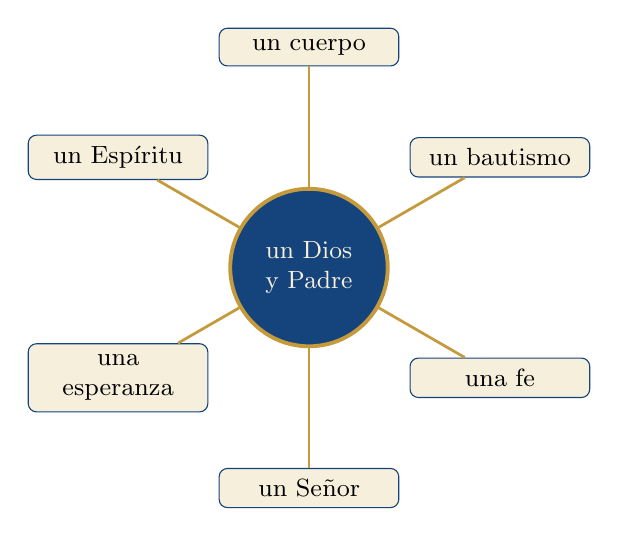
\begin{tikzpicture}[font=\small]
 \node[draw=dorado,line width=1.4pt,fill=azul,text=papiro,circle,minimum size=2.0cm,align=center] (d) at (0,0) {un Dios\\ y Padre};
 \foreach \a/\t in {90/{un cuerpo},150/{un Espíritu},210/{una esperanza},270/{un Señor},330/{una fe},30/{un bautismo}}{
   \node[draw=azul,fill=papiro,rounded corners=3pt,inner sep=4pt,text width=2.0cm,align=center] (n\a) at (\a:2.8) {\t};
   \draw[dorado,line width=1pt] (d)--(n\a);}
\end{tikzpicture}\par
{\footnotesize\color{gris}\textit{Figura 5.} Las siete unidades de Ef 4:4--6. \textit{Nota.} Elaboración propia.}
\end{center}

\subsection{Toda rodilla: Isaías 45 en Filipenses 2}
El texto más fuerte del monoteísmo de Isaías termina con un juramento:

\begin{cita}Mirad a mí, y sed salvos, todos los términos de la tierra, porque yo soy Dios, y no hay más. Por mí mismo hice juramento, de mi boca salió palabra en justicia, y no será revocada: Que a mí se doblará toda rodilla, y jurará toda lengua.\fuente{(Is 45:22--23)}\end{cita}

Pablo lo aplica a Jesús:

\begin{cita}Por lo cual Dios también le exaltó hasta lo sumo, y le dio un nombre que es sobre todo nombre, para que en el nombre de Jesús se doble toda rodilla de los que están en los cielos, y en la tierra, y debajo de la tierra; y toda lengua confiese que Jesucristo es el Señor, para gloria de Dios Padre.\fuente{(Flp 2:9--11)}\end{cita}

El ``nombre que es sobre todo nombre'' es el Nombre del Uno, y el ``uno su nombre'' de Zac 14:9 se cumple en la confesión ``Jesucristo es el Señor''. Todo termina ``para gloria de Dios Padre'': la unidad no se rompe. En Ro 14:11 Pablo cita el mismo Is 45:23 a propósito del juicio de Dios.

\begin{nota}[Precisión]
La lectura de Flp 2:9--11 a la luz de Is 45:22--23 es de Bauckham (2008). Que el ``nombre sobre todo nombre'' sea el Nombre divino es la interpretación mayoritaria; otros lo entienden como el título ``Señor''. Ambas lecturas convergen.
\end{nota}

\subsection{``Yo y el Padre uno somos''}
La confesión de Pablo hunde sus raíces en las palabras de Jesús. En Jerusalén, durante la fiesta de la Dedicación, los judíos le preguntan si él es el Cristo, y Jesús responde hablando de sus ovejas:

\begin{cita}y yo les doy vida eterna; y no perecerán jamás, ni nadie las arrebatará de mi mano. Mi Padre que me las dio, es mayor que todos, y nadie las puede arrebatar de la mano de mi Padre. Yo y el Padre uno somos.\fuente{(Jn 10:28--30)}\end{cita}

\begin{filologia}[Jn 10:30]
\begin{tabular}{@{}L{3.4cm}L{1.6cm}L{9.8cm}@{}}
\grc{ἐγὼ καὶ ὁ πατὴρ} & --- & ``yo y el Padre'': dos sujetos que se nombran por separado. \\[2pt]
\grc{ἕν ἐσμεν} & \grc{εἷς} & ``uno somos'': \grc{ἕν} es neutro, ``una sola cosa''; no dice ``una sola persona'' (que sería masculino, \grc{εἷς}), sino una sola realidad de vida, voluntad y obra. \\
\end{tabular}
\end{filologia}

El argumento de Jesús es el de las dos manos. Nadie arrebata las ovejas de la mano del Hijo (v.~28) y nadie las arrebata de la mano del Padre (v.~29), porque se trata de una sola mano: ``Yo y el Padre uno somos''. La estructura es la misma de Gn 2:24: dos que se nombran por separado y forman una sola unidad. Jesús lo explica en otros pasajes: ``todo lo que el Padre hace, también lo hace el Hijo igualmente'' (Jn 5:19); ``¿No crees que yo soy en el Padre, y el Padre en mí?'' (Jn 14:10). No hay en Dios dos voluntades que negocian, sino una armonía perfecta, y por eso, cuando ora por sus discípulos, Jesús pone esa unidad como modelo:

\begin{cita}La gloria que me diste, yo les he dado, para que sean uno, así como nosotros somos uno.\fuente{(Jn 17:22)}\end{cita}

\subsection{``Una sola carne'': el gran misterio}
Pablo toma el texto del matrimonio y lo lleva hasta Cristo:

\begin{cita}Por esto dejará el hombre a su padre y a su madre, y se unirá a su mujer, y los dos serán una sola carne. Grande es este misterio; mas yo digo esto respecto de Cristo y de la iglesia.\fuente{(Ef 5:31--32)}\end{cita}

Pablo cita Gn 2:24 según la Septuaginta, \grc{οἱ δύο εἰς σάρκα μίαν}, y le da su alcance último: la unión de Cristo con su pueblo. En 1~Corintios vuelve al mismo texto con el mismo verbo: ``¿O no sabéis que el que se une con una ramera, es un cuerpo con ella? Porque dice: Los dos serán una sola carne. Pero el que se une al Señor, un espíritu es con él'' (1~Co 6:16--17). ``Se une'', \grc{κολλώμενος}, es el verbo con que la Septuaginta traduce el \heb{דבק} de Gn 2:24, \grc{προσκολληθήσεται}. La adhesión que Deuteronomio pedía al Dios uno (Dt 10:20) se cumple en la unión con Cristo.

\begin{nota}[Precisión]
La relación entre \grc{κολλάω} en 1~Co 6:17 y \heb{דבק} en Gn 2:24 y Dt 10:20 se apoya en el vocabulario de la Septuaginta; la conexión con Dt 10:20 es observación propia. La autoría paulina de Efesios se discute; 1~Co 6:16--17 dice lo mismo en una carta indiscutida.
\end{nota}

\subsection{La plenitud del Uno en Cristo}
Los demás escritos del Nuevo Testamento dicen lo mismo con otras palabras. Pablo llama a Cristo el único mediador, ``Porque hay un solo Dios, y un solo mediador entre Dios y los hombres, Jesucristo hombre'' (1~Ti 2:5), y formula la tesis de esta serie: ``en él habita corporalmente toda la plenitud de la Deidad'' (Col 2:9). El Uno no se divide en Cristo; en Cristo se da a conocer.

\begin{center}
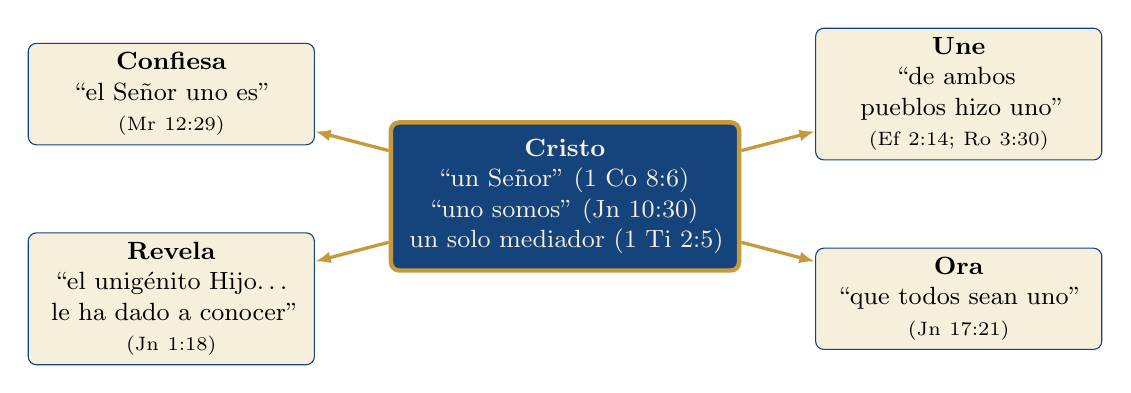
\begin{tikzpicture}[font=\small]
 \node[draw=azul,fill=papiro,rounded corners=3pt,text width=3.4cm,align=center] (a) at (-5.0,1.3) {\textbf{Confiesa}\\ ``el Señor uno es''\\ {\scriptsize(Mr 12:29)}};
 \node[draw=azul,fill=papiro,rounded corners=3pt,text width=3.4cm,align=center] (b) at (-5.0,-1.3) {\textbf{Revela}\\ ``el unigénito Hijo\ldots{} le ha dado a conocer''\\ {\scriptsize(Jn 1:18)}};
 \node[draw=azul,fill=papiro,rounded corners=3pt,text width=3.4cm,align=center] (c) at (5.0,1.3) {\textbf{Une}\\ ``de ambos pueblos hizo uno''\\ {\scriptsize(Ef 2:14; Ro 3:30)}};
 \node[draw=azul,fill=papiro,rounded corners=3pt,text width=3.4cm,align=center] (d) at (5.0,-1.3) {\textbf{Ora}\\ ``que todos sean uno''\\ {\scriptsize(Jn 17:21)}};
 \node[draw=dorado,line width=1.6pt,fill=azul,text=papiro,rounded corners=3pt,text width=4.0cm,align=center,inner sep=6pt] (x) at (0,0) {\textbf{Cristo}\\ ``un Señor'' (1~Co 8:6)\\ ``uno somos'' (Jn 10:30)\\ un solo mediador (1~Ti 2:5)};
 \foreach \n in {a,b,c,d}\draw[dorado,line width=1.2pt,-{Latex[length=2mm]}] (x)--(\n);
\end{tikzpicture}\par
{\footnotesize\color{gris}\textit{Figura 6.} La unidad de Dios en Cristo. \textit{Nota.} Elaboración propia.}
\end{center}

\begin{nota}[Precisión]
En Jn 10:30 ``uno'' es neutro (\grc{ἕν}): ``una sola cosa'', no ``una sola persona''. Juan no es de Pablo, y la autoría de 1~Timoteo y Colosenses se discute; la idea paulina central está en 1~Co 8:6, una carta indiscutida.
\end{nota}

%===================================================================
\section{Aplicación: un corazón no dividido}

La unidad de Dios es incomunicable: solo Dios es Dios. Pero el \emph{Shemá} no termina en el v.~4, sino que continúa con ``y amarás'' (v.~5), y lo que el atributo produce en el creyente es un corazón entero.

\begin{enumerate}
\item \textbf{No claudicar entre dos.} El corazón no se reparte entre Dios y otros ``dioses'', sean el dinero, el prestigio o el poder: ``¿Hasta cuándo claudicaréis vosotros entre dos pensamientos?'' (1~R 18:21). Jesús lo dijo con otras palabras: ``Ninguno puede servir a dos señores\ldots{} No podéis servir a Dios y a las riquezas'' (Mt 6:24).
\item \textbf{Pedir un corazón unido.} La petición del salmista, ``unifica mi corazón'' (Sal 86:11), es la oración que corresponde a un Dios uno.
\item \textbf{Oír cada día.} La confesión se convierte en hábito, como manda el propio texto: ``y hablarás de ellas estando en tu casa, y andando por el camino, y al acostarte, y cuando te levantes'' (Dt 6:7).
\item \textbf{Guardar la unidad.} El Dios uno vive en armonía, y su imagen se reconoce donde dos son uno sin dejar de ser dos: en el matrimonio, ``lo que Dios juntó, no lo separe el hombre'' (Mt 19:6), y en la iglesia, que contradice a su Dios cada vez que se divide. La unidad no se fabrica; se guarda (Ef 4:3), porque Cristo oró por ella: ``así como nosotros somos uno'' (Jn 17:22).
\item \textbf{Ser testigos.} Israel fue llamado a ser testigo del Uno ante las naciones (Is 43:10), y quien confiesa que Dios es uno lleva su Nombre a ``todos los términos de la tierra'' (Is 45:22; Ro 3:29).
\end{enumerate}

Santiago advierte contra una confesión sin corazón:

\begin{cita}Tú crees que Dios es uno; bien haces. También los demonios creen, y tiemblan.\fuente{(Stg 2:19)}\end{cita}

Santiago cita el \emph{Shemá}, \grc{εἷς ἐστιν ὁ θεός}, para mostrar que es posible confesar la unidad de Dios con los labios y tener el corazón dividido: la ortodoxia sin amor es la fe de los demonios. La pregunta que deja el atributo alcanza a cada lector: entre qué dos pensamientos claudica hoy.

%===================================================================
\section{Síntesis}

\begin{tcolorbox}[colback=papiro,colframe=azul,boxrule=1pt,arc=3pt]
Dios es uno: no hay otro fuera de él (Dt 4:35), no tiene igual (Is 46:9) ni se divide (Dt 6:4). Israel lo confiesa cada día en el \emph{Shemá} y lo espera para toda la tierra: ``\SENOR{} será uno, y uno su nombre'' (Zac 14:9). En el Carmelo el pueblo deja de claudicar entre dos (1~R 18:39), y los sabios hacen del ``uno'' la aceptación del Reino y la última palabra de los mártires. Su unidad es armonía perfecta: el Dios que dijo ``hagamos'' (Gn 1:26) hizo de dos ``una sola carne'' (Gn 2:24), y en Cristo se oye: ``Yo y el Padre uno somos'' (Jn 10:30). Pablo confiesa el mismo \emph{Shemá} en Cristo, ``un Dios, el Padre\ldots{} y un Señor, Jesucristo'' (1~Co 8:6), y deduce de él un solo pueblo de judíos y gentiles (Ro 3:30).
\end{tcolorbox}

\begin{center}\small\renewcommand{\arraystretch}{1.3}
\begin{tabular}{@{}L{3.0cm}L{11.4cm}@{}}
\toprule
\textbf{Mirada} & \textbf{Aporte al atributo} \\ \midrule
Hebrea & Dt 6:4--9; 4:35, 39; 10:20; Éx 20:3; Zac 14:9; \emph{ejad} (Gn 2:24), \emph{levad}, \emph{ein od}; Is 43--46; Mal 2:10; Sal 86:10--11; Elías en el Carmelo (1~R 18). \\
Judía & Yugo del Reino (Misná \emph{Berajot} 2:2); prolongar el ``uno'' (\emph{Berajot} 13b); Jacob y sus hijos (\emph{Pesajim} 56a); ``no son dos poderes'' (\emph{Mejiltá}); el \emph{Sifré} y Rashi sobre Zac 14:9; Maimónides; Akiva (\emph{Berajot} 61b); \emph{Neilá}; filacterias y Papiro Nash. \\
Teológica & Dios ``está solo en su excelencia'': la unicidad, la autosuficiencia y el conocimiento por revelación; la unidad como armonía: ``hagamos'' (Gn 1:26), ``una sola carne'' (Gn 2:24), ``uno somos'' (Jn 10:30). \\
Paulina & 1~Co 8:4--6; 6:16--17; Ro 3:29--30; 10:12--13; Ef 4:3--6; 2:14--15; 5:31--32; Flp 2:9--11 con Is 45:23; Col 2:9. \\
\bottomrule
\end{tabular}\par
{\footnotesize\color{gris}\textit{Tabla 7.} Síntesis del capítulo. \textit{Nota.} Elaboración propia.}
\end{center}

\begin{cita}Mas alábese en esto el que se hubiere de alabar: en entenderme y conocerme, que yo soy \SENOR{}, que hago misericordia, juicio y justicia en la tierra; porque estas cosas quiero, dice \SENOR{}.\fuente{(Jer 9:24 [9:23])}\end{cita}

``Que yo soy \SENOR'': conocer a Dios empieza por saber que no hay otro, y por amarlo con un corazón que tampoco tenga otro.

%===================================================================
\section*{Compendio bíblico}
\begin{center}\small\renewcommand{\arraystretch}{1.12}
\begin{tabular}{@{}L{2.2cm}L{5.0cm}|L{2.2cm}L{5.0cm}@{}}
\toprule
Gn 1:26 & ``Hagamos al hombre'' & Mt 19:6 & ``no son ya más dos'' \\
Gn 2:24 & ``serán una sola carne'' & Jn 5:19 & ``también lo hace el Hijo'' \\
Éx 15:11 & ``¿Quién como tú\ldots?'' & Mr 12:29 & ``el Señor uno es'' \\
Éx 20:3 & ``No tendrás dioses ajenos'' & Mr 12:32 & ``uno es Dios, y no hay otro'' \\
Dt 4:35 & ``no hay otro fuera de él'' & Jn 10:30 & ``Yo y el Padre uno somos'' \\
Dt 4:39 & ``arriba en el cielo y abajo'' & Jn 17:3 & ``el único Dios verdadero'' \\
Dt 6:4--5 & ``\SENOR{} uno es'' & Jn 17:22 & ``así como nosotros somos uno'' \\
Dt 32:39 & ``no hay dioses conmigo'' & Ro 3:29--30 & ``Dios es uno'' \\
1~R 18:21 & ``¿Hasta cuándo claudicaréis?'' & Ro 10:12 & ``el mismo que es Señor de todos'' \\
1~R 18:39 & ``¡\SENOR{} es el Dios!'' & Ro 16:27 & ``al único y sabio Dios'' \\
Neh 9:6 & ``Tú solo eres \SENOR'' & 1~Co 8:4--6 & ``un Dios\ldots{} y un Señor'' \\
Sal 86:10--11 & ``sólo tú eres Dios'' & 1~Co 6:17 & ``un espíritu es con él'' \\
Sal 96:5 & ``los dioses\ldots{} son ídolos'' & Gá 3:20 & ``Dios es uno'' \\
Is 43:10--11 & ``Vosotros sois mis testigos'' & Ef 4:4--6 & ``un Dios y Padre de todos'' \\
Dt 10:20 & ``a él seguirás'' & Ef 5:31--32 & ``Grande es este misterio'' \\
Is 44:6 & ``fuera de mí no hay Dios'' & Flp 2:10--11 & ``se doble toda rodilla'' \\
Is 45:5--6 & ``no hay más que yo'' & Col 2:9 & ``toda la plenitud de la Deidad'' \\
Is 45:22--23 & ``a mí se doblará toda rodilla'' & 1~Ti 1:17 & ``al único y sabio Dios'' \\
Is 46:9 & ``nada hay semejante a mí'' & 1~Ti 2:5 & ``un solo Dios, y un solo mediador'' \\
Jer 32:39 & ``un corazón, y un camino'' & 1~Ti 6:15--16 & ``el bienaventurado y solo Soberano'' \\
Zac 14:9 & ``uno su nombre'' & Stg 2:19 & ``Tú crees que Dios es uno'' \\
\bottomrule
\end{tabular}\par
{\footnotesize\color{gris}\textit{Tabla 8.} Compendio bíblico de la unidad de Dios. \textit{Nota.} Textos de la RVR1960.}
\end{center}

%===================================================================
\section*{Glosario}
\begin{description}\setlength{\itemsep}{2pt}
\item[\emph{Alenu}] Oración que cierra los servicios de la sinagoga; termina con Zac 14:9.
\item[\emph{Ani hu}] (\heb{אֲנִי הוּא}). ``Yo (soy) él'' (Dt 32:39; Is 43:10); en la LXX, \grc{ἐγώ εἰμι}.
\item[\emph{Dabaq}] (\heb{דָּבַק}). Adherirse, unirse: al cónyuge (Gn 2:24) y a Dios (Dt 10:20).
\item[\emph{Ed}] (\heb{עֵד}). Testigo; lo forman las letras grandes de Dt 6:4.
\item[\emph{Ein od}] (\heb{אֵין עוֹד}). ``No hay otro'' (Dt 4:35; Is 45:5).
\item[\emph{Ejad}] (\heb{אֶחָד}). Uno, uno solo, el mismo (Dt 6:4; Zac 14:9).
\item[\emph{Heîs}] (\grc{εἷς}). Uno (Mr 12:29; 1~Co 8:6).
\item[\emph{Levad}] (\heb{לְבַד}). Solo, aparte (Neh 9:6; Sal 86:10).
\item[\emph{Mónos}] (\grc{μόνος}). Solo, único (Jn 17:3; Ro 16:27).
\item[\emph{Na'asé}] (\heb{נַעֲשֶׂה}). ``Hagamos'' (Gn 1:26).
\item[\emph{Neilá}] Oración final del Día de la Expiación.
\item[\emph{Ol maljut shamáyim}] ``Yugo del Reino de los cielos'' (Misná \emph{Berajot} 2:2).
\item[\emph{Pasaj}] (\heb{פסח}). Cojear, saltar: ``claudicar'' (1~R 18:21).
\item[\emph{Shemá}] (\heb{שְׁמַע}). ``Oye''; nombre de Dt 6:4--9 y de la oración diaria.
\item[Simplicidad] Término teológico: Dios no está compuesto de partes.
\item[\emph{Tefilín}] Filacterias: cajas pequeñas con Dt 6:4--9 y otros textos (Dt 6:8).
\item[\emph{Yajed}] (\heb{יַחֵד}). Unificar (Sal 86:11).
\item[\emph{Yajid}] (\heb{יָחִיד}). Único, hijo único (Gn 22:2).
\end{description}

\section*{Referencias}
\refapa{Bauckham, R. (2008). \emph{Jesus and the God of Israel: God crucified and other studies on the New Testament's christology of divine identity}. Eerdmans.}
\refapa{Block, D.~I. (2004). How many is God? An investigation into the meaning of Deuteronomy 6:4--5. \emph{Journal of the Evangelical Theological Society, 47}(2), 193--212.}
\refapa{Burkitt, F.~C. (1903). The Hebrew papyrus of the Ten Commandments. \emph{The Jewish Quarterly Review, 15}(3), 392--408.}
\refapa{Carson, D.~A. (2013). \emph{Falacias exegéticas}. Editorial CLIE.}
\refapa{Elbogen, I. (1993). \emph{Jewish liturgy: A comprehensive history} (R.~P. Scheindlin, Trad.). Jewish Publication Society.}
\refapa{Elliger, K., \& Rudolph, W. (Eds.). (1997). \emph{Biblia Hebraica Stuttgartensia} (5.ª ed.). Deutsche Bibelgesellschaft.}
\refapa{Koehler, L., \& Baumgartner, W. (2001). \emph{The Hebrew and Aramaic lexicon of the Old Testament} (M.~E.~J. Richardson, Trad.; Ed. de estudio). Brill.}
\refapa{Maimónides. (s.f.). \emph{Mishné Torá: Yesodé haTorá} [1:7]. Sefaria. https://www.sefaria.org}
\refapa{\emph{Mejiltá de Rabí Yishmael} [Bajódesh 5]. (s.f.). Sefaria. https://www.sefaria.org}
\refapa{Meshel, Z. (2012). \emph{Kuntillet `Ajrud (Ḥorvat Teman): An Iron Age II religious site on the Judah--Sinai border}. Israel Exploration Society.}
\refapa{Milik, J.~T. (1977). \emph{Qumrân grotte 4.II: Tefillin, mezuzot et targums (4Q128--4Q157)} (Discoveries in the Judaean Desert VI). Clarendon Press.}
\refapa{\emph{Misná: Berajot} [2:2; 9:5]. (s.f.). Sefaria. https://www.sefaria.org}
\refapa{Nestle, E., \& Aland, K. (Eds.). (2012). \emph{Novum Testamentum Graece} (28.ª ed.). Deutsche Bibelgesellschaft.}
\refapa{Pink, A. W. (2020). \emph{Los atributos de Dios} (E. Rodríguez Cruz, Trad.). Chapel Library. (Obra original publicada en 1930)}
\refapa{Rahlfs, A., \& Hanhart, R. (Eds.). (2006). \emph{Septuaginta} (Ed. rev.). Deutsche Bibelgesellschaft.}
\refapa{Rashi. (s.f.). \emph{Comentario a la Torá} [Dt 6:4]. Sefaria. https://www.sefaria.org}
\refapa{\emph{Santa Biblia: Reina-Valera 1960}. (1960). Sociedades Bíblicas en América Latina.}
\refapa{Segal, A.~F. (1977). \emph{Two powers in heaven: Early rabbinic reports about Christianity and Gnosticism}. Brill.}
\refapa{\emph{Shulján Aruj: Óraj Jayim} [623:6]. (s.f.). Sefaria. https://www.sefaria.org}
\refapa{\emph{Sifré Devarim} [31]. (s.f.). Sefaria. https://www.sefaria.org}
\refapa{Steinsaltz, A. (Ed.). (2017). \emph{Koren Talmud Bavli: Edición William Davidson} [Berajot 13b; 61b; Pesajim 56a]. Sefaria. https://www.sefaria.org}
\refapa{Steinsaltz, A. (s.f.). \emph{The portion of ``Shema'' (Deuteronomy 6:4--8)}. Steinsaltz Center. \url{https://steinsaltz.org/essay/shema/}}
\refapa{Strong, J. (1890). \emph{The exhaustive concordance of the Bible}. Hunt \& Eaton.}
\refapa{\emph{Targum Ónkelos} [Deuteronomio 6:4]. (s.f.). Sefaria. https://www.sefaria.org}
\refapa{Washer, P. (2021). \emph{Conociendo al Dios vivo} (A. Ávila, A. Valverde y J. Namnún, Trads.). Editorial Legado Bautista Confesional; HeartCry Missionary Society. (Obra original publicada en 2016)}
\refapa{Wright, N.~T. (1991). \emph{The climax of the covenant: Christ and the law in Pauline theology}. T\&T Clark.}

\end{document}
